\section{Background}

\subsection{\texttt{unsafe} keyword in C\#/Rust}
In programming languages like C\# and Rust, pointer operations are explicitly marked as \texttt{unsafe}. This establishes a language-wide boundary to distinguish memory-unsafe code. It is a brilliant concept because it allows users to demonstrate that they can handle APIs correctly, reducing the likelihood of errors. This is especially valuable when working with third-party libraries. In contrast, while C++ employs RAII (Resource Acquisition Is Initialization) for resource management, it does not inherently ensure memory safety. This is because C++ libraries cannot guarantee that users will utilize them correctly 100\% of the time.

The S/P toggle concept discussed in this paper draws inspiration from the \texttt{unsafe} keyword in C\# and Rust. It aims to create a similar boundary, enabling users to safely and correctly operate their devices. At the same time, it ensures that advanced users retain the flexibility they need to perform tasks when necessary.

\subsection{Google's Misplaced Blame on Memory-Unsafe Languages}

Google Chromium has consistently identified memory-unsafe languages, such as C++, as a primary source of its security issues\cite{ruleOf2}. However, this paper contends that, based on this same logic, Google Chrome itself should be deemed fundamentally unsafe. The root cause of these issues extends beyond programming languages, stemming instead from the inherent design of web browsers. As of February 2025, Google Chrome held a dominant 66.3\% share of the global market\cite{statcounter}, with Chromium-based browsers collectively exceeding 80\%. This extensive exposure to arbitrary and untrusted input highlights the fundamental weaknesses in browser architecture.

Every website accessed via a browser is an untrusted remote code execution. While memory-unsafe languages do contribute to some security problems, the larger issue lies in the browser's unavoidable handling of untrusted input, which makes it significantly more susceptible to threats compared to other applications. Following this logic, banning Google Chrome for security concerns for majority of users would align with the rationale used for criticizing C++. If web browsers never existed in the world, the majority of security issues would also disappear, as most devices would no longer face the risks associated with exploiting security vulnerabilities.

\subsection{App Sandboxing}
App sandboxing confines an application's access to system resources and user data within a restricted environment. Apple mandates that all apps in the App Store utilize app sandboxing\cite{appleAppSandbox}. In the Linux ecosystem, app sandboxing has also gained significant traction with technologies like Flatpak, Snap, and AppImage. Similarly, all Android apps are sandboxed by default. The primary advantage of app sandboxing is its ability to enforce app-specific permissions, limiting what each application can do.

However, the drawbacks are substantial. Applications often need to be rewritten to function within sandboxed environments, and this requirement extends to their third-party library dependencies. Many open-source libraries and software lack the necessary updates to adapt to these environments. Additionally, performance can suffer due to the sandbox's isolated nature, which restricts resource sharing. A notorious example is Firefox on Ubuntu, distributed as a Snap package. The Snap version of Firefox has been criticized for slow boot time—sometimes taking up to 20 seconds on an average computer—because it bundles its own version of glibc and other libraries instead of using libraries the distribution itself provides\cite{ubuntuDecline, whatsWrongWithSnaps}.

These sandboxed apps can also create conflicts. Drivers bundled within Snap or Flatpak applications may not align with those provided by the operating system, leading to potential compatibility issues. Furthermore, while the app itself is sandboxed, it still operates within the same memory address space as the kernel. If the kernel has vulnerabilities, app sandboxing cannot prevent kernel-level exploits. This limitation is evident on Android, where malware remains a persistent issue despite widespread app sandboxing. The problem is particularly relevant for mainstream OS kernels like Windows NT, Linux, and Darwin, all of which employ monolithic kernels, not micro kernels.

\subsection{Progressive Web Apps}
Progressive Web Apps (PWAs) are essentially websites that function as applications. Since every platform includes browser support and mainstream web browsers embrace this technology, PWAs are highly versatile. For example, websites like Snaeplayer Music Player or Flow EPUB Reader can be accessed, added to your home screen on any device—be it a phone or PC—and effectively installed as apps. These apps operate using the browser engine already available on the device.

Unlike WebView apps or Electron apps, PWAs do not bundle their own Chromium installation. WebView apps, such as the preinstalled Microsoft Outlook on Windows 11, and Electron apps often duplicate Chromium, which can be resource-intensive. In contrast, PWAs share the same browser engine that the user is already utilizing.

Progressive Web Apps support offline functionality once installed. For instance, Snaeplayer works seamlessly without an internet connection. Furthermore, PWAs can access local files and support features like push notifications, provided the platform-specific apps allow it. They are truly cross-platform, adhering to open web standards, rather than being proprietary technology, making them a robust and inclusive solution for modern app experiences.

Since Progressive Web Apps operate directly within the browser, they inherently function within a sandboxed environment. This design prevents many direct exploits targeting OS APIs and the kernel, providing an additional layer of security compared to other technologies like app sandboxing.

\subsection{WebAssembly}

WebAssembly\cite{WebAssembly2025, 10.1145/3140587.3062363} enables native languages like C and C++ to run on the web, achieving performance levels close to that of native applications. When combined with Progressive Web Apps, it simplifies the development of web-based applications using native languages, making the process more efficient and accessible.

\subsection{Universal Windows Platform}

Microsoft's earlier attempt to establish a walled garden ecosystem relied on its proprietary Universal Windows Platform (UWP) technology. However, Microsoft eventually abandoned UWP in favor of WinUI 3 and other frameworks. One of the key issues with UWP was its severe limitations, particularly due to the lack of a proper permission management system. For example, the developer of Rufus highlighted that UWP could not meet the requirements for accessing USB drives\cite{githubRufusUWP}. Even Microsoft's own documentation for Windows Terminal revealed challenges with UWP, indicating that it was unsuitable for implementation. Moreover, Microsoft's decision to restrict the use of C++ in UWP created additional hurdles, preventing apps like Spotify from porting their cross-platform core engines, which are built in C++ and Assembly, to the UWP ecosystem\cite{microsoftBannedCPlusPlus}.

Although UWP was marketed as a cross-platform solution, developers seeking true cross-platform compatibility require a "universal platform" rather than a "universal Windows platform." They aim to develop for all major operating systems—such as Android, iOS, Linux, and macOS—beyond the Microsoft ecosystem. Progressive Web Apps have proven to be a superior alternative, offering all the capabilities UWP was meant to provide, while adhering to open web standards and supporting seamless functionality across platforms.


\subsection{App Store and Sideloading}
App Stores are now a standard feature across all major operating systems, including Linux GNOME, which offers Flatpak packages. As software distribution channels, App Stores, when properly managed, enhance security by having reviewers evaluate apps before their release—making them more secure than downloading random apps from the internet. However, the significant 30\% revenue cut imposed by platforms like the Apple App Store and Google Play Store remains a widely criticized drawback. Additionally, some apps are either unavailable on these stores or are heavily modified to meet store requirements.

Microsoft is notably more accommodating toward Progressive Web Apps compared to Apple and Google, as they allow PWAs to be distributed through the Microsoft Store. Interestingly, when Steve Jobs unveiled the first-generation iPhone, there was no App Store; instead, he advocated for web apps as the primary application model. Within the framework of this paper, PWA apps should ideally be distributed via a public channel, such as a GitHub repository, while ensuring that a dedicated PWA App Store focuses exclusively on installing PWAs.

\subsection{Antimalware Solutions, Including Microsoft Defender SmartScreen}

Microsoft offers its own anti-malware solution integrated into the Microsoft Edge browser, such as Microsoft Defender SmartScreen, to guard against phishing attacks, malware, and downloading malicious files from the internet. However, much like C++ address sanitizers, these solutions cannot provide absolute guarantees. While they can help detect malicious actors, they cannot completely eliminate security threats. The persistence of malware issues on Windows demonstrates this limitation, despite Microsoft's deployment of multiple layers of security measures, including SmartScreen, Windows Defender, and Windows Firewall.

Third-party anti-malware solutions also attempt to address these challenges, but they too have their own shortcomings. Notable incidents, such as the CrowdStrike outage, underscore the limitations of antivirus solutions across platforms, including Windows, Android, and macOS. These solutions often fail to completely prevent security threats and can sometimes introduce additional problems, as seen in cases like the aforementioned CrowdStrike outage. This highlights the inherent weaknesses in traditional antivirus approaches, especially in complex and evolving threat environments.

\section{Threat Model}
We consider a scenario where users lack technical expertise and may unknowingly engage in risky online behaviors. A typical situation involves users browsing the web with Google Chrome, performing Google Searches, or mistyping URLs, which could inadvertently lead them to malicious or untrusted websites. Upon accessing these sites, users face multiple threats from malicious actors. These attackers may exploit vulnerabilities through techniques like side-channel attacks using JavaScript or WebAssembly, deliver cryptojacking, scareware\cite{scarewareBlocker}, or leverage flaws in the browser's security.

Additionally, users can be tricked into downloading malicious applications designed to extract sensitive data, such as credit card information. Once this occurs, the attackers gain significant control, enabling them to execute harmful actions without restriction. \autoref{fig:threat_model} illustrates the threat model, capturing the various attack vectors and their potential impacts.

\begin{figure*}[h!]
\centering
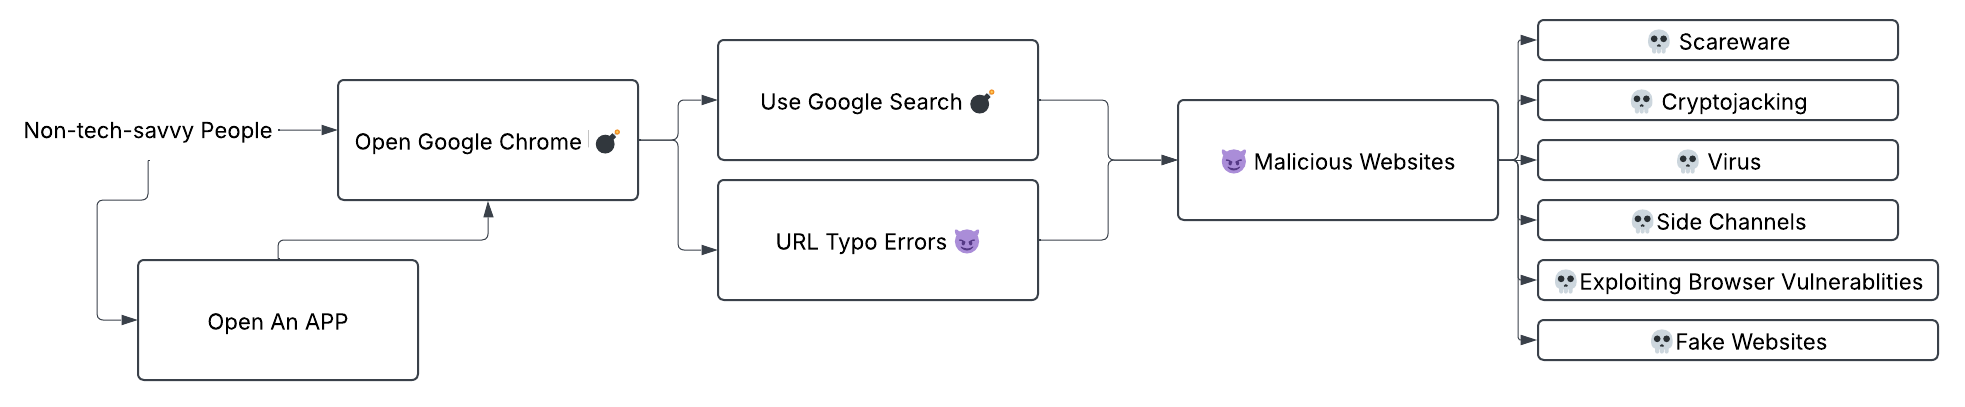
\includegraphics[width=1\textwidth]{threatmodel.png}
\caption{Threat Model: Browsers and Search Engines Considered Unsafe}
\label{fig:threat_model} % Label for referencing the image in the paper
\end{figure*}